\section{A Bridge Circuit}
\label{lab_bridge}

%\makelabheader %(Space for student name, etc., defined in master.tex)

\bigskip

\begin{enumerate}[wide]

\item Measure the resistance of a 10k resistor, and see if you can detect any change in its value if you heat it up between your fingers, being careful not to short circuit the leads.  (You probably can't see any change.)  Be sure you are not accidentally shorting out the resistor with your fingers as you do this.  What is the smallest change in resistance that you could detect in principle, given the precision of your multimeter?

\item Now construct the bridge circuit shown below.  For V1, use your variable DC power supply, $+V$, cranked up as high as it will go.  Let R1 and R2 be 10~k$\Omega$ resistors.  If R3 is 100~k$\Omega$, what should R4 be so that the measured voltage $\Delta V_{ab}$ is zero?  


\begin{center}
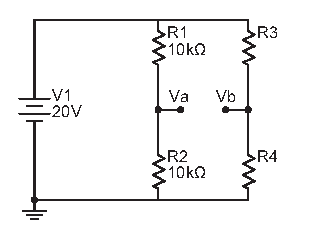
\includegraphics{bridge_circuit/bridge.eps}
\end{center}


\item Draw a circuit showing how how you can insert a trimpot in between R3 and R4, as you did in Lab~\ref{lab_voltage_dividers}, to get $\Delta V_{ab} = 0$ exactly.
	
\item Now see if you can detect a change in $\Delta V_{ab}$ if you warm up R1 with your fingers.  How much does $\Delta V_{ab}$ change by?

\item What is the smallest change in $\Delta V_{ab}$ that you \textit{could} detect, based on the precision of your DMM? \label{part_voltage_measure}

\item Based on your answer to part~\ref{part_voltage_measure}, what is the smallest change in the resistance of R1 that you \textit{could} detect using this bridge circuit?  How does this compare to what you found in part 1?  (This bridge circuit is a good example of a fundamental and powerful principle of experimentation: that doing a difference measurement is usually a lot more sensitive than doing a single measurement directly.)

\item A typical temperature coefficient for a regular-old, smelly-old metal film resistor might be about 0.01\% per degree Celsius.  (That is, the resistance changes by 0.01\% of its value for every 1~$^\circ$C change in temperature.)  From your previous answers, what is the smallest change in temperature that you could detect this way?

\item Suppose you actually wanted to analyze your bridge circuit taking into account the input impedance of the voltmeter.  Is the voltmeter in parallel with another resistor, in series with another resistor, or neither?  Show how you can use a ``Delta to Wye conversion'' (Paynter, pages 170--172) to redraw your bridge circuit as something you could actually analyze.

\end{enumerate}

\textit{Keep your bridge circuit wired up on your breadboards.  We'll be using it again at the end of Lab~\ref{lab_op-amps}.}






